%%%%%%%%%%%%%%%%%%%%%%%%
%
% $Autor: Daanyaal Parvaize, Kreetika Mohanta, Keerti Belmane$
% $Datum: 2025-06-11 20:48:02Z $
% $Pfad: BA25-02-Time-Series/report/Contents/en/Datatransformation.tex
% $Version: 4621 $
%
% !TeX encoding = utf8
% !TeX root = Rename
%
%%%%%%%%%%%%%%%%%%%%%%%%

\chapter{Data Transformation and Data Mining}

\section{Data Transformation}
Data transformation prepares the raw storm data for modeling by ensuring it’s clean, standardized, and formatted for ARIMA and LSTM models. This includes loading and cleaning the data, scaling it for LSTM, and creating sequences for training.

\subsection{Data Loading and Cleaning}
The \texttt{load\_storm\_data} function in \texttt{model\_utils.py} loads the CSV file, detects the wind speed column, handles missing values using forward and backward filling, and ensures a valid \texttt{date} column is present.

\subsection{Data Scaling}
Wind speed values are scaled between 0 and 1 using \texttt{MinMaxScaler} for LSTM training, stabilizing learning and improving performance. The scaler is saved for consistent use during inference.

\subsection{Sequence Creation}
LSTM sequences are generated by transforming the 1D time series into 3D arrays (samples, timesteps, features). This prepares the data in input-output pairs for sequential learning, based on the default sequence length (e.g., 10).

\section{Data Mining}
Data mining extracts patterns from historical wind speed data to forecast future values, using ARIMA for linear trends and LSTM for complex, non-linear dynamics.

\subsection{ARIMA Model}
Implemented in \texttt{train\_models.ipynb}, the ARIMA model captures linear relationships using autoregression (p), differencing (d), and moving average (q). It is suited for stationary time series and is implemented using the \texttt{statsmodels} package.

\subsection{LSTM Model}
Built with TensorFlow and Keras, the LSTM model learns non-linear patterns and long-term dependencies. It uses stacked LSTM layers and a dense output, trained on wind speed sequences with a validation split to monitor overfitting.

\section{Application to the Project}

This project applies time series forecasting techniques to hurricane wind speed data, using either ARIMA or LSTM depending on the context. ARIMA is employed to model linear patterns, while LSTM is chosen for capturing non-linear dependencies. These models provide valuable predictions of future wind speeds to support early warning systems and disaster preparedness.

\section{Hyperparameters}

\subsection{ARIMA Hyperparameters}
\begin{itemize}
	\item \textbf{p, d, q}: Represent the autoregressive (AR), differencing (I), and moving average (MA) terms of the model.
	\item \textbf{Default Settings}: \(p = 2\), \(d = 1\), \(q = 2\). These values are configurable within stable limits to ensure effective model performance.
\end{itemize}

\subsection{LSTM Hyperparameters}
\begin{itemize}
	\item \textbf{Epochs}: Specifies the number of complete training iterations. \textit{Default: 10}
	\item \textbf{Batch Size}: Number of samples processed before the model weights are updated. \textit{Default: 32}
	\item \textbf{Sequence Length}: Defines the number of time steps the model considers. \textit{Default: 10}
\end{itemize}

\section{Input}

The forecasting models are fed with preprocessed data from CSV files. Each input file includes:

\begin{itemize}
	\item A \texttt{wind\_speed} column indicating the primary time series feature.
	\item Date information either in a unified \texttt{date} column or separated into \texttt{year}, \texttt{month}, and \texttt{day}.
\end{itemize}

During preprocessing, missing entries are addressed, and the date formats are standardized to ensure compatibility with time-based indexing.

\section{Training}

\subsection{ARIMA Training}

The ARIMA model is trained using the full dataset, capturing linear temporal dependencies. Once the optimal values of \(p\), \(d\), and \(q\) are determined, the model is fit accordingly to produce stable forecasts.

\subsection{LSTM Training}

The LSTM model is trained using an 80-20 split between training and validation sets. Key training parameters like epochs and batch size govern the learning process, which is visualized through training and validation performance metrics to assess convergence.

\section{Interpretation}

\subsection{ARIMA Forecasts}

ARIMA produces forecasts based on learned linear patterns in the data. Performance is evaluated using RMSE scores, and graphical plots are generated to compare predicted values against the actual observed data.

\subsection{LSTM Forecasts}

LSTM, capable of modeling non-linear trends, provides both forecast outputs and performance diagnostics. These include training-validation loss curves to monitor learning progression and assess overfitting or underfitting.
\section {Output}
\begin{itemize}
	\item Predicted wind speed values for future dates.
	\item Visual output plots, e.g., \texttt{forecast\_plot.png}, for model evaluation.
	\item Serialized model files:
	\begin{itemize}
		\item \texttt{arima\_model.pkl} for ARIMA
		\item \texttt{lstm\_model.h5} for LSTM
	\end{itemize}
	\item Forecast results exported as a CSV file: \texttt{forecast\_results.csv}
\end{itemize}

\section{Visualization of Output}

This section presents the forecast results produced by the ARIMA or LSTM models depending on developer choice. The plot below shows the predicted wind speeds alongside the historical data, allowing for visual comparison of model performance.

\subsection{Diagram-Visualization Of Output}

\begin{figure}[H]
	\centering
	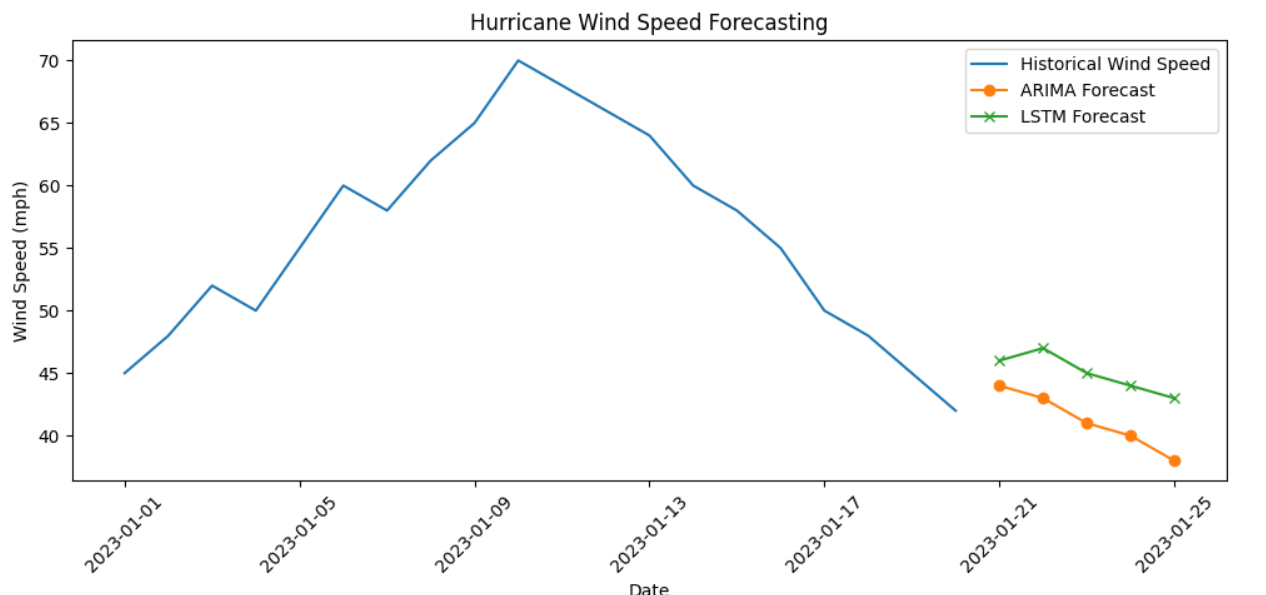
\includegraphics[width=\textwidth]{Images/Output.png}
	\caption{Forecast vs. Actual Wind Speeds}
	\label{fig:forecast_output}
\end{figure}



\begin{figure}[H]
	\centering
	\begin{tikzpicture}[
		node distance=1.5cm and 1.9cm,
		font=\small\sffamily,
		box/.style={
			rectangle, 
			rounded corners, 
			drop shadow={shadow xshift=0.8ex,shadow yshift=-0.8ex,fill=black,opacity=0.15},
			text centered, 
			minimum width=3.8cm, 
			minimum height=1.2cm, 
			align=center,
			font=\small\bfseries,
			text=white,
			fill=#1
		},
		arrow/.style={-{Stealth[length=3mm]}, thick, draw=#1, color=#1},
		inputbox/.style={box=cyan!70!black, font=\small\bfseries},
		preprocessbox/.style={box=orange!85!black},
		modelbox/.style={box=purple!80!black},
		trainbox/.style={box=teal!85!black},
		evalbox/.style={box=olive!90!black},
		outputbox/.style={box=green!75!black, minimum width=5cm},
		]
		
		% Nodes
		\node[inputbox] (input) {Input Data\\\texttt{wind\_speed.csv}};
		\node[preprocessbox, below=of input] (preprocess) {Preprocessing\\(Missing values, Date format)};
		\node[modelbox, below left=0.6cm and 0.9cm of preprocess] (arima) {ARIMA Model\\\textcolor{white}{(p=2, d=1, q=2)}};
		\node[modelbox, below right=0.6cm and 0.9cm of preprocess] (lstm) {LSTM Model\\\textcolor{white}{(Epochs=10, Batch=32)}};
		\node[trainbox, below=of arima] (trainA) {ARIMA Training};
		\node[trainbox, below=of lstm] (trainL) {LSTM Training\\(80-20 Split)};
		\node[evalbox, below=of trainA] (evalA) {ARIMA Forecast\\+ RMSE Evaluation};
		\node[evalbox, below=of trainL] (evalL) {LSTM Forecast\\+ Loss Curves};
		\node[outputbox, below=1cm of $(evalA)!0.5!(evalL)$] (output) {Final Output:\\
			Forecast Values\\
			Visual Plots (e.g. \texttt{forecast\_plot.png})\\
			Saved Models \texttt{arima\_model.pkl}, \texttt{lstm\_model.h5}\\
			CSV Results \texttt{forecast\_results.csv}};
		
		% Arrows with colors
		\draw[arrow=cyan!80!black] (input) -- (preprocess);
		\draw[arrow=orange!80!black] (preprocess) -- (arima);
		\draw[arrow=orange!80!black] (preprocess) -- (lstm);
		\draw[arrow=purple!80!black] (arima) -- (trainA);
		\draw[arrow=purple!80!black] (lstm) -- (trainL);
		\draw[arrow=teal!80!black] (trainA) -- (evalA);
		\draw[arrow=teal!80!black] (trainL) -- (evalL);
		\draw[arrow=olive!90!black] (evalA) -- (output);
		\draw[arrow=olive!90!black] (evalL) -- (output);
		
		% Title above
		\node[align=center, font=\sffamily\Large\bfseries, text=black] at ($(input)+(0,3.5)$) {Project Workflow: Time Series Forecasting \\ \small Using ARIMA and LSTM Models};
		
	\end{tikzpicture}
	\caption{Color-coded visualization of the hurricane wind speed forecasting process}
\end{figure}






\chapter{Survey Note: Detailed Analysis of Data Transformation and Data Mining Application}

This chapter presents a comprehensive analysis of the data preparation and mining methodologies implemented in the hurricane wind speed forecasting project. The analysis is based on the source files: \texttt{app.py}, \texttt{model\_utils.py}, \texttt{developer.py}, \texttt{train\_models.ipynb}, and \texttt{requirements.txt}. Both ARIMA and LSTM models are trained and managed through a user-friendly developer interface and an interactive application frontend.

\section{Data Transformation Analysis}

\subsection{Loading and Cleaning}

Data integrity and continuity are ensured through automatic column detection, systematic handling of missing values, and consistent date formatting. These steps prepare the dataset for reliable analysis and modeling.

\subsection{Scaling and Sequence Creation}

Normalization using \texttt{MinMaxScaler} standardizes the data scale, while reshaping the time series into sequences enables effective training of the LSTM model, contributing to enhanced model stability and accuracy.

\section{Data Mining Analysis}

\subsection{Linear Pattern Extraction via ARIMA}

The ARIMA model leverages classical time series forecasting techniques to capture linear trends and provide interpretable insights into the hurricane wind speed data.

\subsection{Non-linear Dynamics with LSTM}

LSTM networks detect complex, non-linear temporal relationships within the dataset. Model performance is rigorously monitored using validation metrics such as RMSE to ensure forecasting reliability.

\section{Application Overview}

This section details the end-to-end integration of data transformation and mining components within the hurricane wind speed forecasting application developed for this project. Users begin by uploading raw historical wind speed datasets, which are automatically preprocessed through intelligent data cleaning, missing value imputation, and temporal formatting to ensure data integrity.

The application offers a developer interface for configuring hyperparameters specific to either the ARIMA or LSTM models, including lag order selection for ARIMA and sequence length and network architecture for LSTM. Once parameters are set, the models are trained on the processed time series data, leveraging efficient computational routines to balance accuracy with performance.

Forecasts generated by the selected model are output in both tabular and graphical formats within the app frontend, allowing stakeholders to interpret predicted wind speed trends clearly. This facilitates timely decision-making for early warning systems and disaster mitigation strategies. Furthermore, the modular design enables easy extension or substitution of forecasting models as new techniques emerge.
